\usetikzlibrary{arrows.meta,calc}
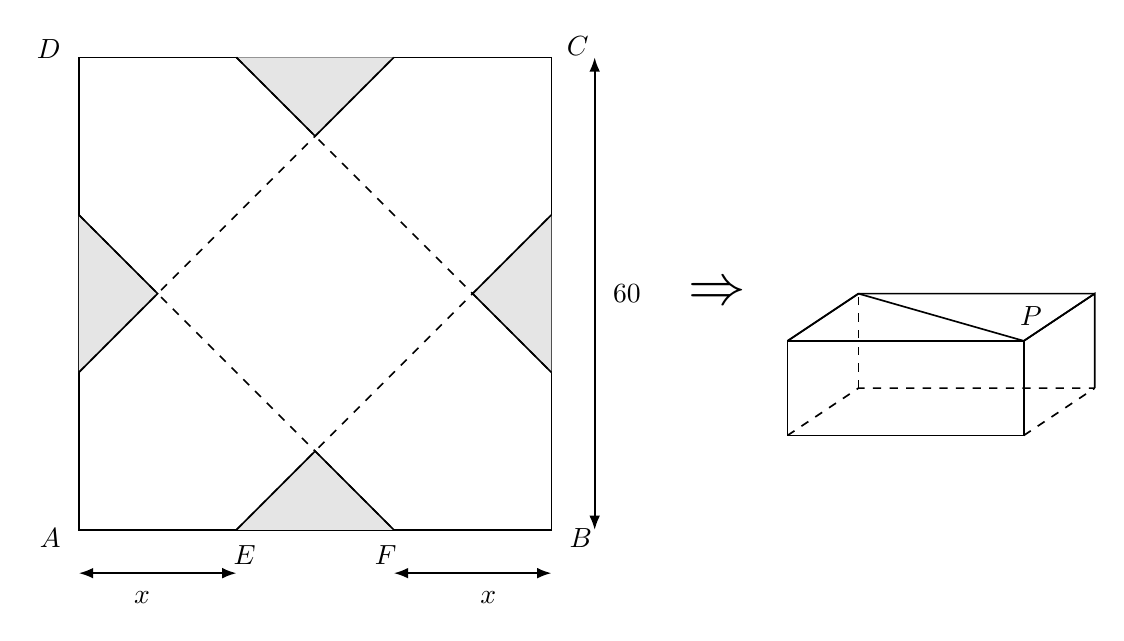
\begin{tikzpicture}[x=1cm,y=1cm,font=\normalsize,line width=.6pt]
% ---- left panel: square net ----
\coordinate (SqBL) at (0,0);
\coordinate (SqBR) at (6,0);
\coordinate (SqTR) at (6,6);
\coordinate (SqTL) at (0,6);
\coordinate (E) at (2.0000000000,0.0000000000);
\coordinate (F) at (4.0000000000,0.0000000000);
\coordinate (T1) at (2.0000000000,6.0000000000);
\coordinate (T2) at (4.0000000000,6.0000000000);
\coordinate (L1) at (0.0000000000,2.0000000000);
\coordinate (L2) at (0.0000000000,4.0000000000);
\coordinate (R1) at (6.0000000000,2.0000000000);
\coordinate (R2) at (6.0000000000,4.0000000000);
\coordinate (ApexB) at (3.0000000000,1.0000000000);
\coordinate (ApexT) at (3.0000000000,5.0000000000);
\coordinate (ApexL) at (1.0000000000,3.0000000000);
\coordinate (ApexR) at (5.0000000000,3.0000000000);
\draw[solid] (SqBL) -- (SqBR) -- (SqTR) -- (SqTL) -- cycle;
% shaded cut triangles (gray)
\fill[gray!20] (T1) -- (T2) -- (ApexT) -- cycle;
\fill[gray!20] (L1) -- (L2) -- (ApexL) -- cycle;
\fill[gray!20] (R1) -- (R2) -- (ApexR) -- cycle;
% solid cut edges
\draw[solid] (T1) -- (ApexT) -- (T2);
\draw[solid] (L1) -- (ApexL) -- (L2);
\draw[solid] (R1) -- (ApexR) -- (R2);
\fill[gray!20] (E)--(ApexB)--(F)--cycle;
\draw[solid] (E)--(ApexB)--(F);
% dashed fold diamond (box bottom)
\draw[dashed] (L1)--(T2) (L2)--(F);
\draw[dashed] (T1)--(R1) (E)--(R2);
% labels with clearance
\node[left,xshift=-3pt,yshift=3pt] at (SqTL) {$D$};
\node[right,xshift=2pt,yshift=4pt] at (SqTR) {$C$};
\node[left,xshift=-3pt,yshift=-3pt] at (SqBL) {$A$};
\node[right,xshift=3pt,yshift=-3pt] at (SqBR) {$B$};
\node[below,yshift=-2.0pt,xshift=3.0pt] at (E) {$E$};
\node[below,yshift=-2.0pt,xshift=-3.0pt] at (F) {$F$};
% x dimensions at bottom
\draw[{Latex[length=1.8mm]}-{Latex[length=1.8mm]}] (0,-0.55) -- (2,-0.55);
\node[below,yshift=-3pt] at (0.8,-0.55) {$x$};
\draw[{Latex[length=1.8mm]}-{Latex[length=1.8mm]}] (4,-0.55) -- (6,-0.55);
\node[below,yshift=-3pt] at (5.2,-0.55) {$x$};
% 60 dimension at right
\draw[{Latex[length=1.8mm]}-{Latex[length=1.8mm]}] (6.55,0) -- (6.55,6);
\node[right,xshift=3pt] at (6.55,3) {$60$};
% ---- arrow between panels ----
\node at (8.1,3) {\huge $\Rightarrow$};
% ---- right panel: low box ----
\begin{scope}[shift={(9,1.2)},x=1cm,y=1cm]
\coordinate (fbl) at (0,0);
\coordinate (fbr) at (3,0);
\coordinate (ftr) at (3,1.2);
\coordinate (ftl) at (0,1.2);
\coordinate (bbl) at (0.9,0.6);
\coordinate (bbr) at (3.9,0.6);
\coordinate (btr) at (3.9,1.8);
\coordinate (btl) at (0.9,1.8);
\coordinate (Pv) at (3.0000000000,1.2000000000);
\draw[solid] (fbl) -- (fbr) -- (ftr) -- (ftl) -- cycle;
\draw[solid] (ftr) -- (btr) -- (bbr);
\draw[solid] (ftl) -- (btl) -- (btr);
\draw[solid] (btl) -- (ftl);
\draw[dashed] (fbl) -- (bbl) -- (bbr);
\draw[dashed] (bbl) -- (btl);
\draw[dashed] (fbr) -- (bbr);
% top converging edges to P (folded corners meet)
\draw[solid] (ftl) -- (Pv);
\draw[solid] (ftr) -- (Pv);
\draw[solid] (btl) -- (Pv);
\draw[solid] (btr) -- (Pv);
\node[above right,xshift=-5pt,yshift=2pt] at (Pv) {$P$};
\end{scope}
\end{tikzpicture}
